\setcounter{secnumdepth}{-1}

\chapter{Transmission chain blocks}

\section{Baseband representation}

By looking at the block diagram of the transmission chain \ref{fig:blockDiagram}, one can see we never move the baseband signal to the carrier frequency. As the simulation runs on a computer, using the bandpass representation of the signal would require much more samples as the sampling frequency would need to be at least twice the carrier frequency. By simulating the chain in baseband, the minimal sampling frequency is reduced to the symbol rate in order to have at least one sample per symbol. \\
Because the signal is oversampled, the sampling frequency is then equal to the symbol rate multiplied by the oversampling factor. \\

\section{Modulation and Demodulation}

After generating N random bits, they are modulated. This allows to send fewer symbols than the number of bits. We chose QAM modulation as it combines ASK and PSK. Depending on the number of bits per symbol ($N_{\text{bps}}$), the number of bits sent ($N$) had to be chosen such that  $N / N_{\text{bps}} \in \mathbb{N}$. \\
Figure \ref{fig:QAMComparison} compares the modulation the constellation diagrams obtained for QAM-16 and QAM-64. As the constellations points are more spaced on the left, QAM-16 is less prone to a wrong demodulation (when noise will be added). This comes at the cost of a lower bitrate: for the same symbol rate, QAM-64 will send 6 bits while QAM-16 only send 4. It clearly shows a compromise between reliability and capacity. \\

\begin{figure}[H]
    \centering
    \begin{subfigure}[b]{0.45\linewidth}
        \centering
        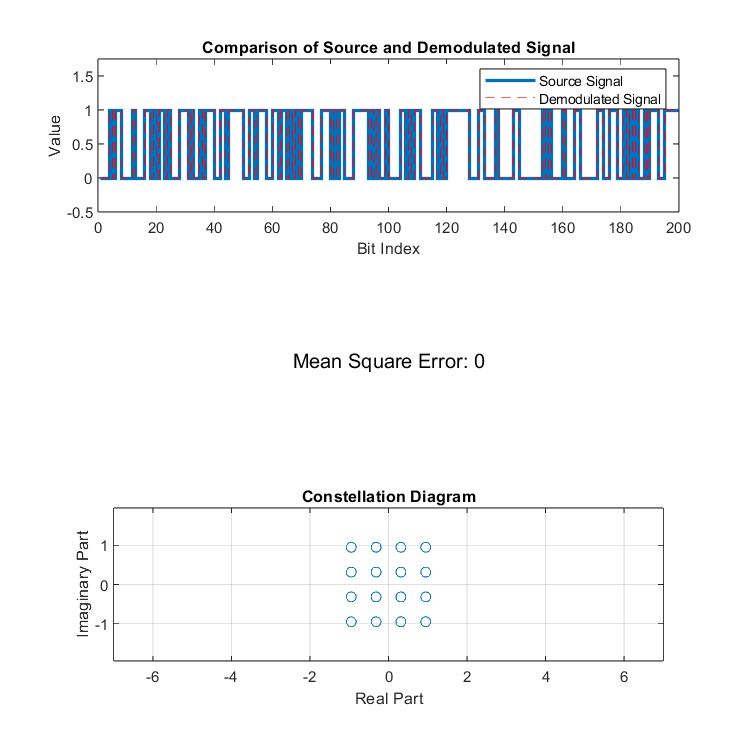
\includegraphics[width=\linewidth]{modulation16.png}
        \caption{QAM-16 modulation}
        \label{fig:QAM16}
    \end{subfigure}
    \hfill
    \begin{subfigure}[b]{0.45\linewidth}
        \centering
        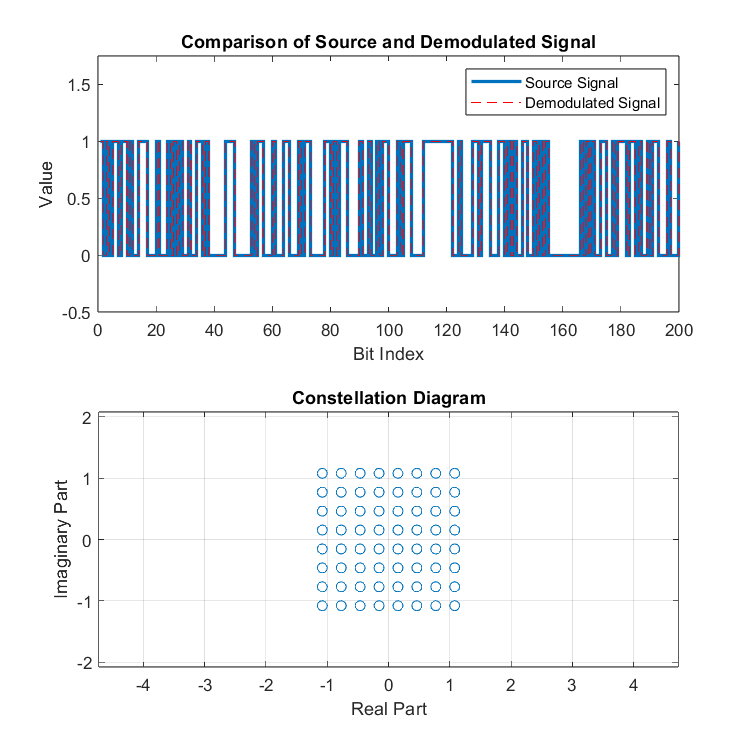
\includegraphics[width=\linewidth]{modulation64.png}
        \caption{QAM-64 modulation}
        \label{fig:QAM64}
    \end{subfigure}
    \caption{Comparison of QAM modulations, where the mean square error is computed between the transmitted and received bitstream}
    \label{fig:QAMComparison}
\end{figure}

\section{Pulse shaping}

With modulation only, the bandwidth of the transmitted signal is infinite. This is problematic as it could interfere with neighboring channels. A filtering is applied to resolve this but the chosen filter must respect two other constraints: it must cancel inter-symbol interference (ISI) and must maximize the SNR. \\
The raised cosine filter is chosen as it limits the bandwidth and cancels ISI. To maximize the SNR, it is applied as a matched filter by using the square root of it at the transmitter and at the receiver. \\
The time domain and frequency domain representation of the raised cosine filter is shown in Figure \ref{fig:raisedCosine}. Figure \ref{fig:pulseShaping} shows how the signal is shaped in the time domain and how there is indeed no ISI. Finally, the spectrum of the transmitted signal is plotted in figure \ref{fig:shapedSpectrum} where the frequency band is limited to $[-3, 3]$MHz. \\

\begin{figure}[H]
    \centering
    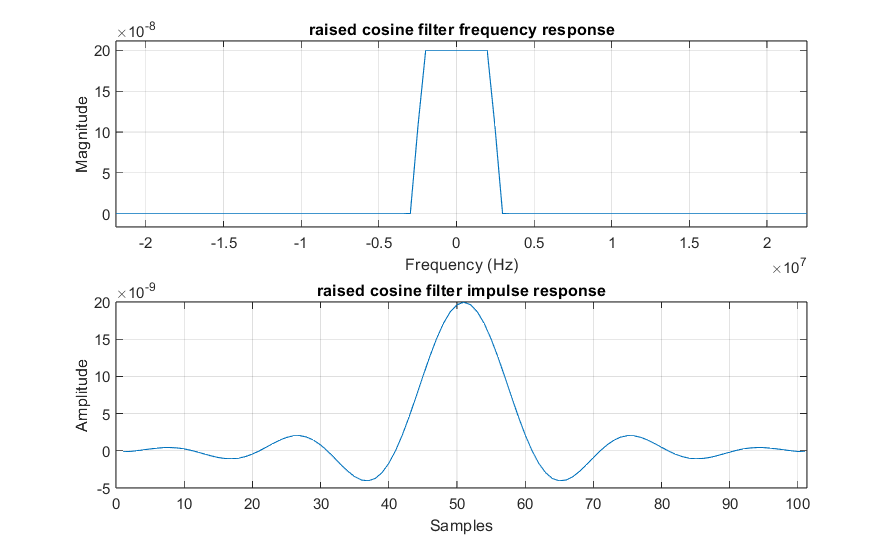
\includegraphics[width=0.9\linewidth]{raisedCosine.png}
    \caption{Time and frequency domain representation of the raised cosine filter}
    \label{fig:raisedCosine}
\end{figure}

\begin{figure}[H]
    \centering
    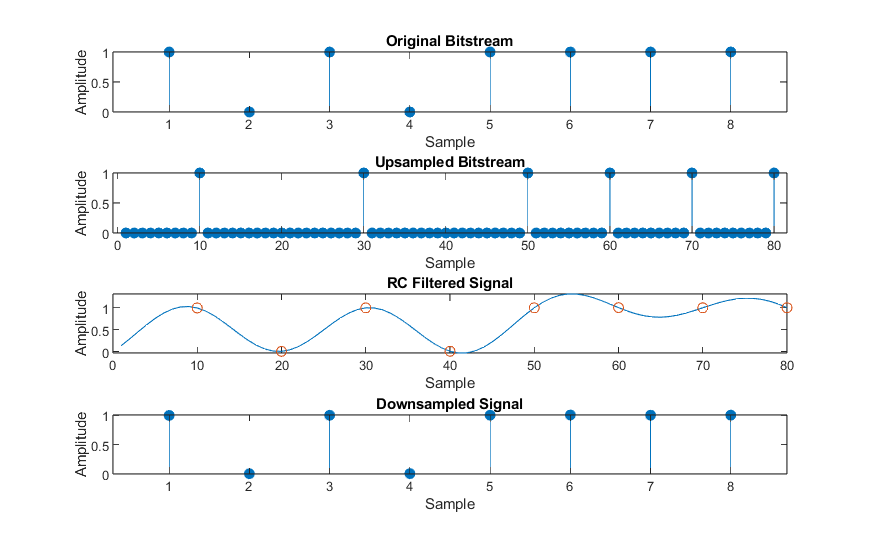
\includegraphics[width=0.9\linewidth]{pulseShaping.png}
    \caption{Pulse shaping with a raised cosine filter}
    \label{fig:pulseShaping}
\end{figure}

\begin{figure}[H]
    \centering
    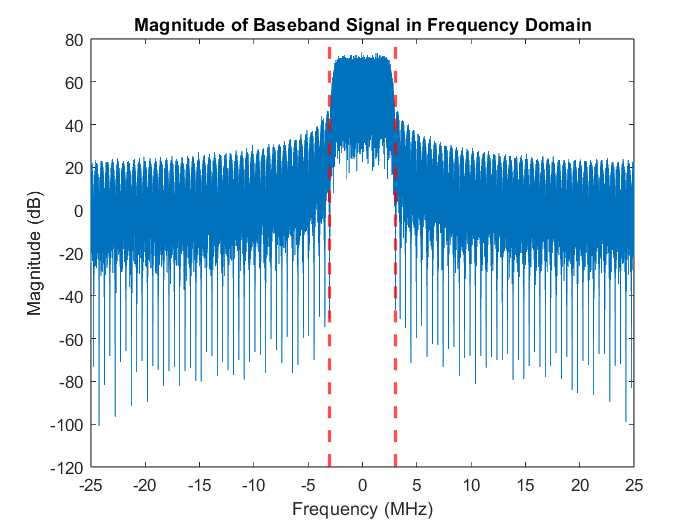
\includegraphics[width=0.9\linewidth]{shapedSpectrum.png}
    \caption{Spectrum of the transmitted signal after pulse shaping}
    \label{fig:shapedSpectrum}
\end{figure}

\section{Noise addition}

\section{About the simulation}



